\begin{Problem}
	Es seien
	\[
		A:=\begin{pmatrix} 10 & -31 & -60 & 180 \\ 0 & 3 & -21 & 63 \\ 2 & -8 & 0 & 0 \\ 10 & -31 & -60 & 183 \end{pmatrix},~B:=\begin{pmatrix} 1 & 3 & 0 & 0 \\ 2 & 3 & 1 & 0 \\ 1 & 0 & 0 & 2 \\ 0 & 0 & 1 & 0 \end{pmatrix} 
	.\] 
	\begin{parts}
		\item Bestimmen Sie die Determinante von $B$ direkt mit dem Laplace’schen Entwicklungssatz  
		\item Bestimmen Sie die Determinante von $A$ einmal, indem Sie den Laplace’schen Entwicklungssatz direkt anwenden, und einmal, indem Sie vorher eine geschickte Zeilenumformung durchführen.   
		\item Wie verhält es sich mit dem Aufwand jetzt gegenüber letzter Woche? Beschreiben Sie eine Strategie zum geschickten Berechnen von Determinanten bei Matrizen geeigneter Struktur.  
	\end{parts}
\end{Problem}
\begin{proof}
	\begin{parts}
	\item Laplaceentwicklung durch die vierte Spalte:
		\begin{align*}
			\text{det}(B)=&-2
			\begin{vmatrix}
				1 & 3 & 0 \\ 2 & 3 & 1 \\ 0 & 0 & 1
			\end{vmatrix}\\
			=&-2(1)
			\begin{vmatrix}
				1 & 3 \\ 2 & 3
			\end{vmatrix}\\
			=&-2(1)(3-6)\\
			=&6
		\end{align*}
	\item Laplaceentwicklung durch die dritte Zeile
		\begin{align*}
			\text{det}(A)=&2
			\begin{vmatrix}
				-31 & -60 & 180 \\ 3 & -21 & 63 \\ -31 & -60 & 183
			\end{vmatrix}
			+8
			\begin{vmatrix}
				10 & -60 & 180 \\ 0 & -21 & 63 \\ 10 & -60 & 183
			\end{vmatrix}\\
			\begin{vmatrix}
				-31 & -60 & 180 \\ 3 & -21 & 63 \\ -31 & -60 & 183
			\end{vmatrix}=&(-31)
			\begin{vmatrix}
				-21 & 63 \\ -60 & 183
			\end{vmatrix}
			+60
			\begin{vmatrix}
				3 & 63 \\ -31 & 183
			\end{vmatrix}
			+180
			\begin{vmatrix}
				3 & -21 \\ -31 & -60
			\end{vmatrix}\\
			=&(-31)(-63)+60(2502)+180(-311)\\
			=&2493\\
			\begin{vmatrix}
				10 & -60 & 180 \\ 0 & -21 & 63 \\ 10 & -60 & 183
			\end{vmatrix}=&10
			\begin{vmatrix}
				-21 & 63 \\ -60 & 183
			\end{vmatrix}
			+10
			\begin{vmatrix}
				-60 & 180 \\ -21 & 63
			\end{vmatrix}\\
			=&-630\\
			\text{det}(A)=-54
		\end{align*}
		Jetzt führen wir eine Zeilenumformung durch.
		\[
			\begin{pmatrix} 10 & -31 & -60 & 180 \\ 0 & 3 & -21 & 63 \\ 2 & -8 & 0 & 0 \\ 10 & -31 & -60 & 183 \end{pmatrix} \xrightarrow{R_4-R_1}\begin{pmatrix} 10 & -31 & -60 & 180 \\ 0 & 3 & -21 & 63 \\ 2 & -8 & 0 & 0 \\ 0 & 0 & 0 & 3 \end{pmatrix} 
		.\] 
		Laplaceentwicklung durch die dritte Zeile:
		\begin{align*}
			\text{det}(A)=&3
			\begin{vmatrix}
				10 & -31 & -60 \\ 0 & 3 & -21 \\ 2 & -8 & 0
			\end{vmatrix}\\
			=&3(10)
			\begin{vmatrix}
				3 & -21 \\ -8 & 0
			\end{vmatrix}+3(2)
			\begin{vmatrix}
				-31 & -60 \\ 3 & -21
			\end{vmatrix}\\
			=&-3(10)(21\cdot 8)+3(2)(31\cdot 21+60\cdot 3)\\
			=&-54
		\end{align*}
	\item Die Arbeit ist einfacher. Man sollte, wenn möglich, die Zeilen bzw. Spalten umformen, bis eine Zeile bzw. Spalte so viel wie möglich null Einträge hat.\qedhere
	\end{parts}
\end{proof}
\begin{Problem}
	Es sei $K$ ein Körper. F\"{u}r eine Matrix $A\in\text{Mat}(n\times n,K)$ und $k\le n$ bezeichnen wir mit $A[1:k,1:k]$ die Untermatrix von $A$, die aus den ersten $k$ Spalten der ersten $k$ Zeilen besteht, dh. f\"{u}r
	\[
		A=\begin{pmatrix} 1 & 2 & 3 \\ 4 & 5 & 6 \\ 7 & 8 & 9 \end{pmatrix} 
	\]
	wäre
	\[
		A[1:2,1:2]=\begin{pmatrix} 1 & 2 \\ 4 & 5 \end{pmatrix} 
	.\] 
	\begin{parts}
	\item Beweisen Sie: Sind $L,R,D\in \text{Mat}(n\times n,K)$ der Reihe nach eine linke untere Dreiecksmatrix mit ausschließlich Einsen auf der Diagonalen, eine rechte obere Dreiecksmatrix mit ausschließlich Einsen auf der Diagonalen und eine Diagonalmatrix, deren Diagonaleinträge alle $\neq 0$ sind, dann gilt f\"{u}r $A=LDR$ und alle $k=1,\dots, n$ $\text{det}(A[1:k,1:k])\neq 0$.
	\item Beweisen Sie: Ist $A\in \text{Mat}(n\times n,K)$ eine Matrix, f\"{u}r die f\"{u}r alle $k\le n$ $\text{det}(A[1:k,1:k])\neq 0$ gilt, ann gibt es eine linke untere Dreiecksmatrix $L$ mit ausschließlich Einsen auf der DIagonalen, eine rechte obere Dreiecksmatrix $R$ mit ausschließlich Ensen auf der Diagonalen und eine Diagonalmatrix $D$, deren Diagonaleinträge alle $\neq 0$ sind, sodass $A=LDR$ gilt.
	\item Erklären Sie, was dieses Resultat mt elementaren Zeilenumformungen zu tun hat.
	\end{parts}
\end{Problem}

\begin{Problem}
	Es sei $A\in \text{Mat}(n\times n, K)$ eine invertierbare Matrix. Zeigen Sie, dass die folgenden Aussagen äquivalent sind.
	\begin{parts}
		\item $A$ ist invertierbar.
		\item $\text{det}(A)\neq 0$.
		\item Die Spalten von $A$ sind linear unabhängig.
		\item Der Rang von $A$ ist $n$.
		\item Die Zeilen von $A$ sind linear unabhängig.
		\item Die Abbildung $L_A:K^n\to K^n,x\to Ax$ ist surjektiv.
		\item Die Abbildung  $L_A$ ist injektiv.
		\item Die Abbildung $L_A$ ist bijektiv.
		\item Es gilt $\text{ker}(A)=\{0\} $.
		\item Jedes Gleichungssystem der Form $Ax=b$ mit $b\in K^n$ ist eindeutig lösbar.
		\item Es gilt $Ax=0$ nur f\"{u}r $x=0$.
	\end{parts}
\end{Problem}
\begin{proof}
Hier ist der Plan
\begin{center}
	\begin{tikzpicture}[ implies/.style={thick,double,double equal sign distance,-implies}, iimplies/.style={thick,double,double equal sign distance,implies-implies},scale=2]  
		\draw (0,0) node (A){(a)};
		\draw (1,0) node (H) {(h)};
		\draw (2,1) node (F) {(f)};
		\draw (2,-1) node (G) {(g)};
		\draw (3,0) node (D) {(d)};
		\draw (4,1) node (C) {(c)};
		\draw (4,-1) node (E) {(e)};
		\draw[iimplies] (A) -- (H);
		\draw[implies] (H) -- (F);
		\draw[implies] (H) -- (G);
		\draw[implies] (G) -- (D);
		\draw[implies] (D) -- (C);
		\draw[iimplies] (C) -- (E);
		\draw[implies] (F) -- (D);
		\draw (2,2) node (B) {(b)};
		\draw[implies] (C) -- (B);
		\draw[implies] (B) -- (A);
		\draw (2,-2) node (I) {(i)};
		\draw (1,-2) node (K) {(k)};
		\draw (1,-1) node (J) {(j)};
		\draw[iimplies] (G) -- (I);
		\draw[iimplies] (I) -- (K);
		\draw[iimplies] (H) -- (J);
	\end{tikzpicture}
\end{center}
\begin{enumerate}
	\item Per Definition ist $A$ invertierbar genau dann, wenn die Abbildung invertierbar ist. Abbildungen sind invertierbar genau dann, wenn die bijektiv sind.
	\item Bijektive Abbildungen sind sowohl injektiv als auch surjektiv.
	\item Per Definition ist der Rang die Dimension des Bildraums. Sei jetzt die Abbildung surjektiv. Dann ist $\text{Bild}(L_A)=K^n$ mit dimension $n$, also (f) $\implies$ (d).
	\item Sei jetzt $L_A$ injektiv. Dann ist $\text{dim}(L_A(K^n))=\text{dim}(K^n)=n$, also Dimension des Bilds ist gleich Dimension des Definitionsbereiches.
	\item Rang ist $n$ genau dann, wenn die Spalten linear unabhängig sind (Zeilenstufenform).
	\item Spalten sind linear unabhängig genau dann wenn Zeilen linear unabhängig sind (Zeilenrang = Spaltenrang, im Skript).
	\item Per letzte Übungsblatt: Linear unabhängige Spalten $\implies$ $\text{det}(A)\neq 0$. 
	\item (g) $\iff$ (i) per Satz 5.3.10 (Homomorphiesatz). 
	\item (i) $\iff$ (k) per Definition des Kerns.
	\item Bijektivität liefert eine eindeutige Lösung. Surjektivität liefert eine Lösung, Injektivität liefert Eindeutigkeit.\qedhere
\end{enumerate}
\end{proof}

\begin{Problem}
	Es sei $V$ ein endlich dimensionaler $K$-Vektorraum. Beweisen oder widerlegen Sie:
\begin{parts}
\item Sind $U,V\subseteq V$ Unterräume mit $U\not\subseteq W$ und $W\not\subseteq U$, dann ist $U\cup W$ kein Unterraum von $V$.
\item Sind $U,W\subset V$ Unterräume mit $\text{dim}(U)=\text{dim}(W)=2$ und gilt $\text{dim}(V)=3$, dann gilt $U=W$ oder $\text{dim}(U\cap W)=1$.
\item Sind $U,W$ Unterräume von $V$ und sind $\phi:U\to K,\psi:W\to K$ lineare Abbildungen, dann gibt es eine lineare Abbildung $\Psi:U+W\to K$ mit $\Psi(u)=\phi(u)$ f\"{u}r alle $u\in U$ und $\Psi(w)=\psi(w)$ f\"{u}r $w\in W$.
\item Ist $U\subseteq V$ ein Unterraum, dann gibt es genau einen Unterraum $W\subseteq V$ mit $U\oplus W=V$.
\end{parts}
\end{Problem}
\begin{proof}
	\begin{parts}
	\item Wahr. Per Definition gibt es $u\in U$, aber $u \not\in W$ und $w\in W$, aber $w\not\in U$. Falls $U\cup W$ ein Unterraum wäre, würde $u+w\in U\cup W$, also entweder $u+w\in U$ oder $u+w\in W$. Sei $u+w=v\in U$. Dann gilt $w=v-u\in U$, also $w\in U$, ein Widerspruch. Analog bekommt man ein Widerspruch falls $u+v\in W$.
	\item Wahr. Aus $U\cap W\subseteq U$ gilt $\text{dim}(U\cap W)\le 2$. Wenn es $2$ wäre, ist $U=U\cap W$. Daraus folgt: $U=W$.

	Wir müssen daher nur den Fall $\text{dim}(U\cap W)=0$ ausschließen. In diesem Fall: Sei $u_1,u_2$ eine Basis von $U$ sowie $w_1,w_2$ eine Basis von $W$. Da $\text{dim}(U\cap W)=0$, st $U\cap W=\{e\} $ und $\{u_1,u_2,w_1,w_2\} $ ist linear unabhängig. Dadurch haben wir $4$ linear unabhängige Vektoren in einem Raum mit Dimension $3$, ein Widerspruch.
\item Falsch. Sei $U=W$ und $U\ni V\in W$. Sei jetzt $\phi(u)\neq \psi(u)$. Dann kann nicht gleichzeitig $\phi(u)=\Psi(u)$ und $\psi(u)=\Psi(u)$ gelten.
\item Falsch. Sei $V=\R^3$ und $U=\text{span}((1,0,0)^T,(0,1,0)^T)$. Wir betrachten $V=\text{span}((0,0,1)^T)$ und $V'=\text{span}((0,1,1)^T)$.

	Es ist klar, dass $V\cap U=V'\cap U=\{(0,0,0)\} $, also die direkte Summe ist wohldefiniert. Per Definition ist $\R^3=V\oplus U$. Jedoch gilt 
	\[
		\begin{pmatrix} 0 \\ 0 \\ 1 \end{pmatrix} = \underbrace{\begin{pmatrix} 0 \\ 1 \\ 1 \end{pmatrix}}_{\in V'} - \underbrace{\begin{pmatrix} 0 \\ 1 \\ 0 \end{pmatrix} }_{\in V}
	\]
	also $\left(0,0,1 \right)^T\in V'\oplus U$. Daraus folgt, dass $V\oplus U\subseteq V'\oplus U$. Dann ist $V'\oplus U=\R^3$.\qedhere
	\end{parts}
\end{proof}

\begin{Problem}
	Es sei $V=(\Z / 2\Z)^3$.
	\begin{parts}
	\item Bestimmen Sie alle eindimensionalen Unterräume von $V$.
	\item Bestimmen Sie anschließend für alle eindimensionalen Unterräum $U,W\subseteq V$ mit $U\neq W$ den Rang $U\oplus W$. 
	\item Begründen Sie, dass Sie nun alle ein- und zweidimensionalen Unterräume von V gefunden haben.
	\item Visualisieren Sie die Struktur der Unterräume, in dem sie für jeden Unterraum einen Punkt in der Ebene festlegen und zwei Unterräume $U,V$ genau dann mit einem Pfeil $U\to W$ verbinden, wenn $U\subset W$ gilt.
	\item Wie können Se anhand Ihres Bildes $U\cap W$ bzw. $U+W$ ablesen?
	\end{parts}
\end{Problem}
\begin{proof}
	\begin{parts}
	\item So ein Unterraum enthält zumindest ein Vektor, der nicht null ist. Weiter muss der Unterraum gleich der Span des Vektors sein. Da der Körper $\Z / 2\Z$ ist, enthält er nur $2$ Elemente, $1$ und $0$. Sei $v\in (\Z / 2\Z)^3$. Dann ist $1v=v$ und $0v=0$, also ein $1$-dimensionaler Unterraum enthält ein Vektor und der Nullvektor.

		Dann gibt es, f\"{u}r alle $v\in V$, ein Unterraum $\{0, v\} $ der Dimension 1.
	\item Wir betrachten $v,w\in V$ mit $v\neq 0$ und die entsprechenden Unterräume $V$ bzw. $W$. Der Unterraum enthält $v+w$, also er enthält mindestens $\{0,v,w,v+w\} $. Dies ist aber alles. Die Vektoren erzeugen keine neuen Vektoren, da $v+v=w+w=0$ und daraus $(v+w)+v=v+v+w=w$ usw.
	\item In (a) wurde es schon begründet, warum alle eindimensionale Unterräume hier sind. Die zweidimensionale Unterräme müssen durch 2 Vektoren gespannt werden, z.B $u$ und $w$. Wir können dann der Unterraum als direkte Summe von die entsprechenden Unterraume konstruieren.
	\item In der Legende schreiben wir nur die nicht null Vektoren, es versteht sich also, dass die Unterräme der Nullvektor enthalten.

		\begin{center}
			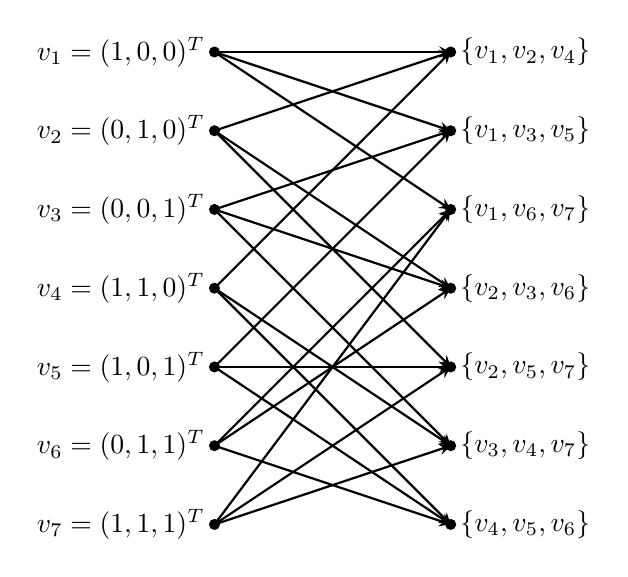
\begin{tikzpicture}[arw/.style={thick,-stealth}]
				\foreach \x in {1, ..., 7}
			\fill (0, \x) circle (2pt);
			\draw (0,7) node[anchor=east] {$v_1=(1,0,0)^T$};
			\draw (0,6) node[anchor=east] {$v_2=(0,1,0)^T$};
			\draw (0,5) node[anchor=east] {$v_3=(0,0,1)^T$};
			\draw (0,4) node[anchor=east] {$v_4=(1,1,0)^T$};
			\draw (0,3) node[anchor=east] {$v_5=(1,0,1)^T$};
			\draw (0,2) node[anchor=east] {$v_6=(0,1,1)^T$};
			\draw (0,1) node[anchor=east] {$v_7=(1,1,1)^T$};
			\foreach \x in {1, ...,7}
		\fill (3,\x) circle (2pt);
			\draw (3,7) node[anchor=west] {$\{v_1,v_2,v_4\} $};
			\draw[arw] (0,7) -- (3,7);
			\draw[arw] (0,6) -- (3,7);
			\draw[arw] (0,4) -- (3,7);
			\draw (3,6) node[anchor=west] {$\{v_1,v_3,v_5\} $};
			\draw[arw] (0,7) -- (3,6);
			\draw[arw] (0,5) -- (3,6);
			\draw[arw] (0,3) -- (3,6);
			\draw (3,5) node[anchor=west] {$\{v_1,v_6,v_7\} $ };
			\draw[arw] (0,7) -- (3,5);
			\draw[arw] (0,2) -- (3,5);
			\draw[arw] (0,1) -- (3,5);
			\draw (3,4) node[anchor=west] {$\{v_2,v_3,v_6\} $ };
			\draw[arw] (0,6) -- (3,4);
			\draw[arw] (0,5) -- (3,4);
			\draw[arw] (0,2) -- (3,4);
			\draw (3,3) node[anchor=west] {$\{v_2,v_5,v_7\} $ };
			\draw[arw] (0,6) -- (3,3);
			\draw[arw] (0,3) -- (3,3);
			\draw[arw] (0,1) -- (3,3);
			\draw (3,2) node[anchor=west] {$\{v_3,v_4,v_7\} $ };
			\draw[arw] (0,5) -- (3,2);
			\draw[arw] (0,4) -- (3,2);
			\draw[arw] (0,1) -- (3,2);
			\draw (3,1) node[anchor=west] {$\{v_4,v_5,v_6\} $ };
			\draw[arw] (0,4) -- (3,1);
			\draw[arw] (0,3) -- (3,1);
			\draw[arw] (0,2) -- (3,1);
			\end{tikzpicture}
		\end{center}
	\item $U\cap W$: Wir suchen die Punkte, die einen auf sowohl $U$ als auch $W$ richteten Pfeil haben.
		
		$U+W$: Wir suchen Pfeile von $U$ und $W$, die sich auf dem gleichen Punkt richtet. Das Punkt ist also $U+W$.\qedhere 
	\end{parts}
\end{proof}
